\documentclass{xmgr}
\usepackage{ gensymb }
\usepackage{listings}
\usepackage[table]{xcolor}
\lstset{language=C}
\setcounter{secnumdepth}{5}
\usepackage{paralist}
\definecolor{orange}{rgb}{1,0.5,0}

\makeatletter
\newcommand\footnoteref[1]{\protected@xdef\@thefnmark{\ref{#1}}\@footnotemark}
\makeatother

\author   {Daniel Sienkiewicz}
\nralbumu {206358}
\email    {daniel@sienkiewicz.ovh}


\title    {Projekt komputera samochodowego bazujący na systemie mikrokomputera Intel Galileo}
\date     {2015}
\miejsce  {Gdańsk}

\opiekun  {dr inż. Janusz Młodzianowski}

\begin{document}

\begin{abstract}
Celem pracy jest stworzenie komputera pokładowego do samochodu, w którego skład wchodzi: \begin{enumerate}
\item Mikrokomputer Intel Galileo Gen 1, 
\item Ekran dotykowy FTDI VM800, 
\item Oprogramowanie,
\item Kamerka cofania.
\end{enumerate}

\end{abstract}
\keywords{Intel Galileo, 
 $I^2C$,
 SPI, 
 C, 
 Arduino,
 GPIO,
 FTDI EVE,
 VM800}
\maketitle

%================WPROWADZENIE=====================
\chapter{Wprowadzenie}
\section{Cele}
Celem pracy jest budowa oraz oprogramowanie komputera pokładowego do samochodu. Komputer powinien móc wczytać z czujników temperaturę panującą w silniku, na zewnątrz oraz w środku samochodu. Ponadto powinien on móc zapisać aktualną pozycję \emph{GPS} na karcie pamięci microSD oraz umożliwić korzystanie z kamerki cofania lub inteligentnego lusterka wstecznego. Komunikacja użytkownika z komputerem będzie odbywała się poprzez użycie ekranu dotykowego \emph{FTDI EVE VM800}.
\section{Założenia}
Do wykonania komputera wykorzystano: \emph{Intel Galileo} wraz z niezainstalowanym oprogramowaniem \emph{Linux YOCTO}, \emph{Arduino IDE}, lokalizator \emph{GPS} służący do podawania aktualnej pozycji dzięki której obliczana zostaje droga przebyta przez samochód, kamerka internetowa służąca jako czujnik cofania oraz inteligentne lusterko wsteczne oraz symulator samochodu. Aktualnie komputer nie będzie zamontowany do fizycznego samochodu więc do tych celów zbudowany został symulator składający się z podstawowych czujników takich jak: guziki służące za czujnik zapięcia pasów/zamknięcia drzwi, potencjometry służące za czujniki temperatury oraz \emph{I/O expander PCF8574N} pozwalający na komunikację z \emph{Intel Galileo}. Na komputerze nie będzie wyświetlana aktualna prędkość ani przebieg ponieważ nawet w najnowszych samochodach nie jest to dostępna opcja. Dane te są dostępne na zegarach samochodowych więc nie ma potrzeby powtarzania tej informacji.
\section{Plan pracy}

Pierwszy rozdział opisuje podstawowe cele oraz założenia projektu.

Druga część pracy przedstawia architekturę projektu wraz z jego opisem funkcjonalnym. Opisuję również mechanizmy komunikacji systemu mikroprocesorowego z otoczeniem.

W następnym rozdziale przedstawiony zostaje pomysł implementacji oraz proces tworzenia niezbędnej do obsługi symulatora samochodu biblioteki pozwalającej na komunikację poprzez \emph{I/O Expander PCF8574N} z \emph{Intel Galielo}. Zostaje tutaj również opisany proces tworzenia oprogramowania ekranu dotykowego FTDI EVE VM800.

Ostatnia część pracy przedstawia pomysły  możliwych rozszerzeń projektu o dodatkowe moduły oraz funkcjonalności w zależności od potrzeb użytkownika.
%================KONIEC WPROWADZENIE=====================

%================ARCHITEKTURA=====================
\chapter{Architektura}
\subsection{Mechanizmy komunikacji systemu mikroprocesorowego z otoczeniem}
\subsubsection{Porty}

Porty są jednym z najbardziej podstawowych interfejsów. Najczęściej dzieli się je na porty:
\begin{enumerate}
	\item Cyfrowe
	\item Analogowe
\end{enumerate}

Porty cyfrowe charakteryzują się możliwością przyjęcia lub wysłania sygnału binarnego (1 - jest sygnał, 0 - sygnału nie ma). Z kolei porty analogowe mogą przesyłać sygnały nawet 10 bitowe. Każdy z portów może działać w jednym  z dwóch trybów: wejścia - oczekiwać na przyjęcie danych od urządzenia zewnętrznego oraz wyjścia - wysyłać dane do urządzenia zewnętrznego. 


W środowisku Arduino aby obsłużyć port analogowy wystarczy:
\begin{lstlisting}[label=bot-dirs-alg,caption=Obsługa portu analogowego w środowisku Arduino]
int val = 0;
int analogPin = A1;	
pinMode(analogPin, OUTPUT);
val = analogRead(analogPin);
pinMode(analogPin, INPUT);
analogWrite(ledPin, val);
\end{lstlisting}

oraz odpowiednio dla portu cyfrowego:
\begin{lstlisting}[label=bot-dirs-alg,caption=Obsługa portu cyfrowego w środowisku Arduino]
int val = 0;
int digitalPin = 1;	
pinMode(digitalgPin, OUTPUT);
val = digitalRead(analogPin);
pinMode(digitalPin, INPUT);
digitalWrite(digitalPin, HIGH);
\end{lstlisting}

\subsubsection{Przerwania}

Przerwania są to bezpośrednie funkcje systemu lub sprzętu ułatwiające komunikację ze światem zewnętrznym. Część z nich jest zarezerwowana przez system lecz część z nich jest wolna do wykorzystania dla programisty. Przerwania możemy podzielić na trzy podstawowe rodzaje:

\begin{enumerate}
	\item Programowe
	\item Sprzętowe
	\begin{enumerate}
		\item Maskowalne (NMI)
		\item Niemaskowalne (INTR)
	\end{enumerate}
	\item Wyjątek
\end{enumerate}

Przerwania programowe wywołuje się za pomocą komendy INT XX gdzie XX oznacza numer przerwania zadeklarowanego w tablicy wektorów przerwań, która jest tworzona przy każdorazowym starcie systemu. Przerwanie to może przyjąć wartości do 255 i są one zarezerwowane przez procesor oraz użytkownika.

Przerwanie sprzętowe jest to rodzaj przerwań wywoływanych przez urządzenia wejścia/wyjścia lub zgłaszane przez procesor. Zostają one wywołane niezależnie w określonych przypadkach. Przerwania te dzielimy na maskowalne oraz niemaskowalne. Główna różnica między nimi polega na możliwości zablokowania przerwań maskowalnych podczas gdy przerwania niemaskowalne muszą zostać obsłużone. Przykładem przerwania niemaskowalnego INT2 czyli popularny blue screen of death.

Ostatnim rodzajem przerwań są wyjątki. Wywoływane są podczas napotkania przez procesor błędów oraz niepowodzeń. Arduino oczywiście obsługuje przerwania. Ich obsłga jest bardzo prosta:
W środowisku Arduino aby obsłużyć port analogowy wystarczy:

\begin{lstlisting}[label=bot-dirs-alg,caption=Obsługa przerwań sprzętowych w środowisku Arduino]
attachInterrupt(pinInt, funcName, mode);
\end{lstlisting}
gdzie pinInt jest to pin na którym Arduino będzie nasłuchiwało na przerwanie, funcName jest to nazwa funkcji który zostanie wykonana gdy przerwanie zostanie zgłoszone, mode - jest to określenie kiedy sygnał może być uznany za przerwanie.

\subsubsection{Odpytywanie w pętli}
Jednym z najprostszych metod pozyskania danych z mikro kontrolera jest jego odpytywanie w nieskończonej pętli.Jest to najmniej efektywny sposób ponieważ cały czas zajmuje niepotrzebnie zasoby sprzętu niepotrzebnymi zapytaniami.

\begin{lstlisting}[label=bot-dirs-alg,caption=Odpytywanie w nieskończonej pętli w środowisku Arduino]
void loop() {
	funcName();
	delay(1000);
}
\end{lstlisting}

\subsubsection{Timer}
\begin{lstlisting}[label=bot-dirs-alg,caption=Przykładowe użycie timer w środowisku Arduino]
#include <TimerOne.h>
Timer1.initialize(500000);
Timer1.attachInterrupt(funcName, 500000);
\end{lstlisting}

%================KONIEC ARCHITEKTURA=====================

%================IMPLEMENTACJA=====================
\chapter{Implementacja}
\subsection{Intel Galileo}
Intel Galileo jest  to mikro kontroler oparty na 32-bitowym procesorze Intel® Quark SoC X1000 i taktowaniu 400MHz. Został on wyposażony w 14 pinów cyfrowych (w tym 6 pinów mogących pełnić funkcję PWM) oraz 6 pinów cyfrowych.Każdy z tych pinów jest w stanie operować napięciem max 5V. Bardzo dużym atutem Galileo jest wbudowana karta sieciowa, port RS-232 oraz port USB oraz slot karty microSD. Galileo może być używane w dwóch trybach - trybie w pełni kompatybilnym z Arduino oraz w trybie z zainstalowanym systemem operacyjnym (np. Linux).
\begin{figure}[!h]
    \centering
    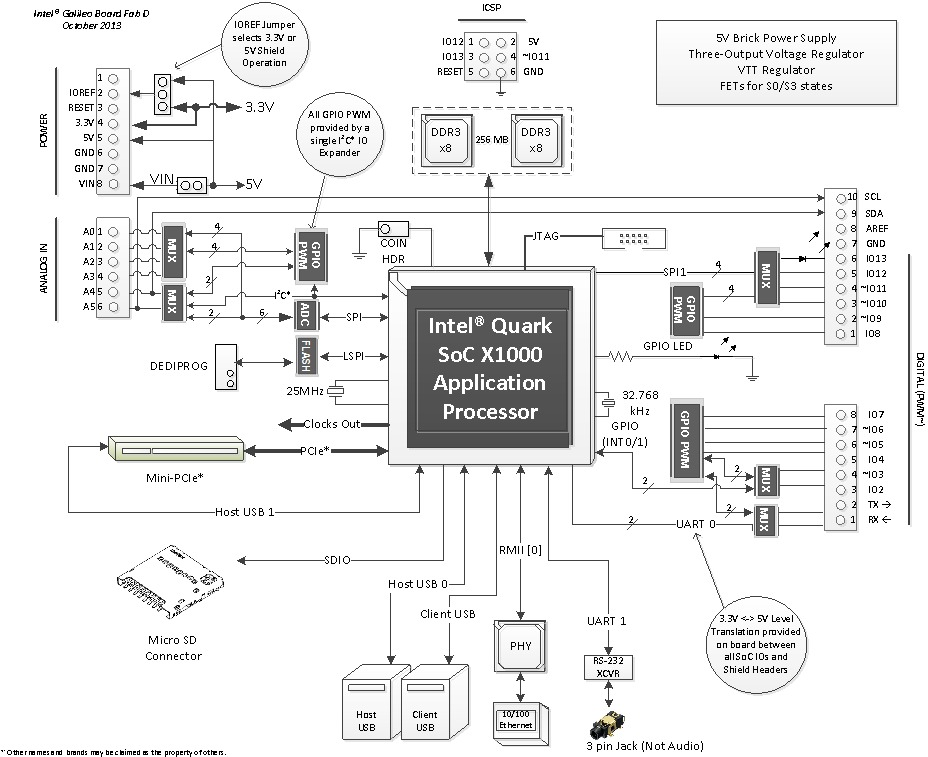
\includegraphics[height=0.8\textwidth]{images/IntelGalileoLogicSchematics.jpg}
    \caption{Schemat logiczny układu Intel Galileo\label{IntelGalileoLogicSchematics}}
    \source{\url{https://www.arduino.cc/en/ArduinoCertified/IntelGalileo}}
\end{figure}

%ŹRÓDŁO: https://www.arduino.cc/en/ArduinoCertified/IntelGalileo

\section{Protokół komunikacyjny $I^2C$}
\emph{$I^2C$} jest szeregowym interfejsem służącym do przesyłania danych między urządzeniami elektrycznymi. 

Podstawową cechą \emph{$I^2C$} jest wykorzystywanie dwóch linii służących do komunikacji: linia \emph{SDA\footnote{Serial Data Line}} oraz linia \emph{SCL\footnote{Serial Clock Time}}. Każdą transmisję danych należy rozpocząć sygnałem \emph{START} oraz zakończyć sygnałem \emph{STOP}. Dane wysyłane są od najstarszego do najmłodszego bitu oraz otrzymanie każdego z nich musi być potwierdzone przez odbiornik. Należy również pamiętać aby każdą komunikację z urządzeniem rozpocząć i zakończyć ustawiając linie \emph{SDA} oraz \emph{SCL} w stan nieaktywny (HIGH). Podstawowe zalety protokołu:
\begin{enumerate}
	\item Połączenia składają się tylko z dwóch linii co znacznie ogranicza liczbę kabli wychodzących z urządzenia
	\item Duża dostępność sprzętu w sklepach
	\item Transmisja jest odporna na zakłócenia zewnętrzne
	\item Bez większych problemów można dodawać oraz odejmować układy korzystające z magistrali
\end{enumerate}
Odbieranie danych rozpoczyna się wysłaniem sygnału START, a następnie zaadresowaniu urządzenia. Kolejnym krokiem jest ustalenie tryby (w tym wypadku read) oraz odczytanie potwierdzenia. Po wykonaniu tych czynności można rozpocząć odbierania danych, które należy zakończyć wysłaniem sygnału \emph{STOP}.

\begin{figure}[!h]
    \centering
    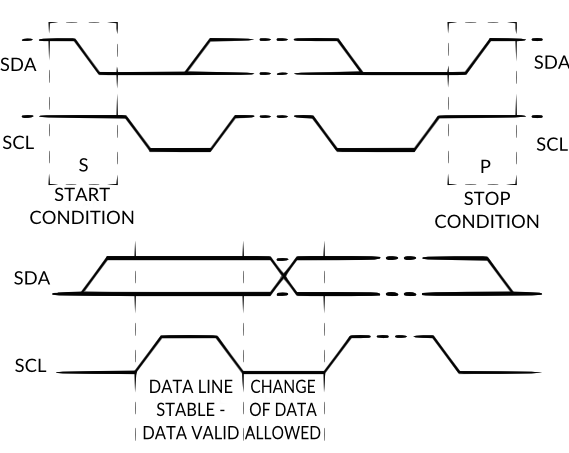
\includegraphics[height=0.4\textheight]{images/i2c.png}
    \caption{Przebieg czasowy protokołu $I^2C$}
    \source{\url{http://www.byteparadigm.com/applications/introduction-to-i2c-and-spi-protocols/}}
\end{figure}

\subsection{Użycie protokołu $I^2C$ na przykładzie I/O Expander PCF8574N}
Wygenerowanie sygnału \emph{START} polega na ustawieniu linii \emph{SDA} oraz \emph{SCL} w stan niski (LOW), a wygenerowanie sygnału \emph{STOP} polega na ustawieniu linii \emph{SDA} oraz \emph{SCL} w stan wysoki (HIGH).

Adresowanie urządzenia odbywa się poprzez wysłanie wysłanie pojedynczych bitów adresu (pamiętając o kolejności MSB->LCB) oraz wygenerowanie impulsu zegara.
\begin{lstlisting}[label=bot-dirs-alg,caption=Adresowanie urządzenia $I^2C$ na przykładzie PCF8574N]
for(m = 0x80; m; m >>= 1){
    if(adres & m)         
      digitalWrite(sda, HIGH);
    else
      digitalWrite(sda, LOW);
        
   digitalWrite(scl, HIGH);
   digitalWrite(scl, LOW); 
}
\end{lstlisting}
Po otrzymaniu potwierdzenia na linii \emph{SDA} można zacząć czytać dane przesyłane z urządzenia.

\begin{figure}[!h]
    \centering
    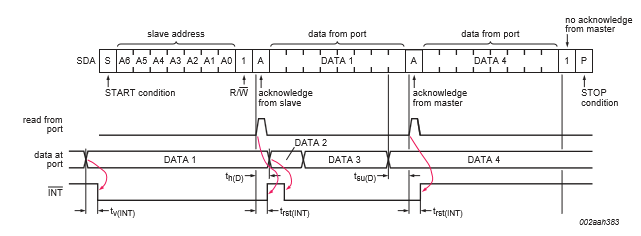
\includegraphics[height=0.2\textheight]{images/read_i2c.png}
    \caption{Przykładowy schemat odbierania danych poprzez $I^2C$ na przykładzie PCF8574N\label{$I^2C$}}
    \source{Karta katalogowa I/O Expander PCF8574N}
\end{figure}

Podobnie jak odbieranie danych, wysyłanie danych należy rozpocząć od wysłania sygnału \emph{START} wraz z adresem urządzenia oraz trybem (write). Po otrzymaniu potwierdzenia można rozpocząć wysyłanie danych w odpowiednich dla urządzenia paczkach x-bitowych. Po wysłaniu każdej z nich otrzymamy potwierdzenie. Na zakończenia transmisji należy wysłać sygnał \emph{STOP}.

\begin{figure}[!h]
    \centering
    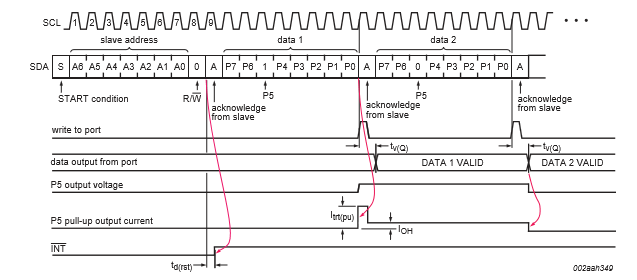
\includegraphics[height=0.2\textheight]{images/write_i2c.png}
    \caption{Przykładowy schemat wysyłania danych poprzez $I^2C$ na przykładzie PCF8574N\label{$I^2C$}}
    \source{Karta katalogowa I/O Expander PCF8574N}
\end{figure}
\subsection{Problemy z bibliotekami}
\subsection{Własna implementacja $I^2C$}
\subsection{Własna biblioteka do komunikacji poprzez $I^2C$ dla Intel Galileo}
\section{Protokół komunikacyjny SPI}
Kolejnym przykładem interfejsu szeregowego jest protokół SPI\footnote{Serial Peripherial Interface}. Składa się on z trzech podstawowych linii - dwóch służących do przesyłania danych w przeciwnych kierunkach oraz jednej z sygnałem taktującym synchronizującym transfer danych. 

Linia MISO\footnote{Master In Slave Out} jest linią wejścia danych dla urządzenia nadrzędnego (master), a wyjściem dla urządzenia podrzędnego (slave), linia MOSI\footnote{Master Out Slave In} jest wyjściem dla urządzenia master, a wejściem dla slave. Linia SCK\footnote{Serial Clock} jest wejściem taktującym. Sygnał taktujący jest zawsze generowany przez układ master. Transmisja danych na obydwu liniach jest zawsze dwukierunkowa i odbywa się jednocześnie - nadanie danych na linii MISO wiąże się z nadaniem danych na linii MOSI. Nie zawsze jednak nadane dane niosą ze sobą informację - najczęściej nadawane informacje płyną w jedną stronę podczas gdy w tym samym czasie wysyłane zostają puste dane. Parametry CPOL\footnote{Clock Polarity} oraz CPHA\footnote{Clock Phase} określają polaryzację oraz fazę sygnału zegarowego.

\begin{figure}[!h]
    \centering
    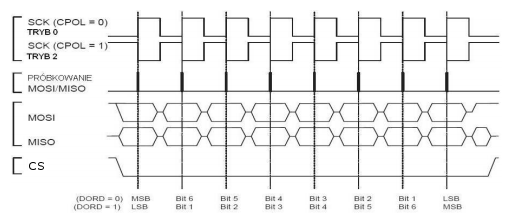
\includegraphics[height=0.3\textheight]{images/spi.png}
    \caption{Przebiegi czasowe interfejsu SPI dla sygnału zegarowego o CPHA=0}
    \source{\url{http://castor.am.gdynia.pl/~dorra}}
\end{figure}

\begin{figure}[!h]
    \centering
    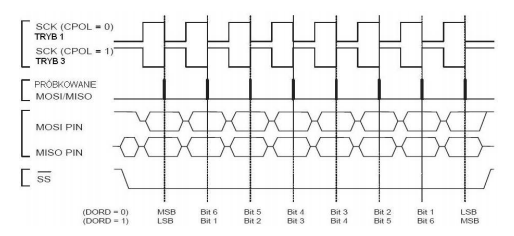
\includegraphics[height=0.3\textheight]{images/spi2.png}
    \caption{Przebiegi czasowe interfejsu SPI dla sygnału zegarowego o CPHA=1}
    \source{\url{http://castor.am.gdynia.pl/~dorra}}
\end{figure}

%ŻRÓDŁO: http://castor.am.gdynia.pl/~dorra/pliki/Magistrale%20%20-%20podstawy%20teoretyczne.pdf

\begin{table}[!h]
\begin{tabular}{|c|c|c|c|} \hline
 & Zbocze pierwsze & Zbocze ostatnie & Tryb SPI \\ \hline
CPOL = 0, CPHA = 0 & Pobieranie (narastanie) & Pobieranie (opadanie) & 0 \\ \hline
CPOL = 0, CPHA = 1 & Ustawianie (narastanie) & Ustawianie (opadanie) & 1 \\ \hline
CPOL = 1, CPHA = 0 & Pobieranie	(opadanie) & Pobieranie (narastanie) & 2\\ \hline
CPOL = 1, CPHA = 1 & Ustawianie (opadanie) & Ustawianie (narastanie) & 3 \\ \hline
\end{tabular}
\caption{Tryby reakcji na fazę i biegunowość sygnału zegarowego}
\source{\url{http://atmega32.republika.pl/22.htm}}
\end{table}

\subsection{Komunikacja poprzez protokół SPI}
Komunikacja zawsze przebiega dwustronnie (duplex\footnote{Nadawanie i odbieranie informacji odbywa się w obu kierunkach}). Zmienia taktu zegara z niskiego na wysoki daje możliwość odczytania danych z linii MISO i jednocześnie wysłania danych na linię MOSI. W przypadku zmiany taktu zegara z wysokiego na niski dane zostają wysłane poprzez linię MISO i jednocześnie odczytane z linii MOSI.

\subsection{VM800}
\emph{FDTI EVE VM800} jest to wyświetlacz dotykowy wraz z wbudowanym kontrolerem audio. Podstawowe cechy urządzenia:
\begin{enumerate}
	\item Pojedynczy układ scalony dla wyświetlacza oraz kontrolera Audio
	\item Rozdzielczość ekranu do 512 x 512 pikseli
	\item 262 tys. kolorów
	\item Możliwość wygładzania krawędzi
	\item Możliwość komunikacji poprzez użycie interfejsu $I^2C$ lub SPI
	\item Wbudowane widgety dostępne dla użytkownika
	\item Zakres pracy wyświetlacza: $-40^{\circ} C$ do $85^{\circ} C$ 
\end{enumerate}

%Źródło: http://www.ftdichip.com/EVE.htm oraz http://www.ftdichip.com/Products/ICs/FT800.html
\section{Założenia funkcjonalne projektu}
Najważniejszym założeniem funkcjonalnym była komunikacja z zestawem czujników, które mogą być zamontowane w samochodzie. czytanie z czujników, pisanie do ekranu, czytanie z ekranu
włączanie i wyłączanie systemu

\subsection{Symulator samochodu}
\begin{figure}[!p]
    \centering
    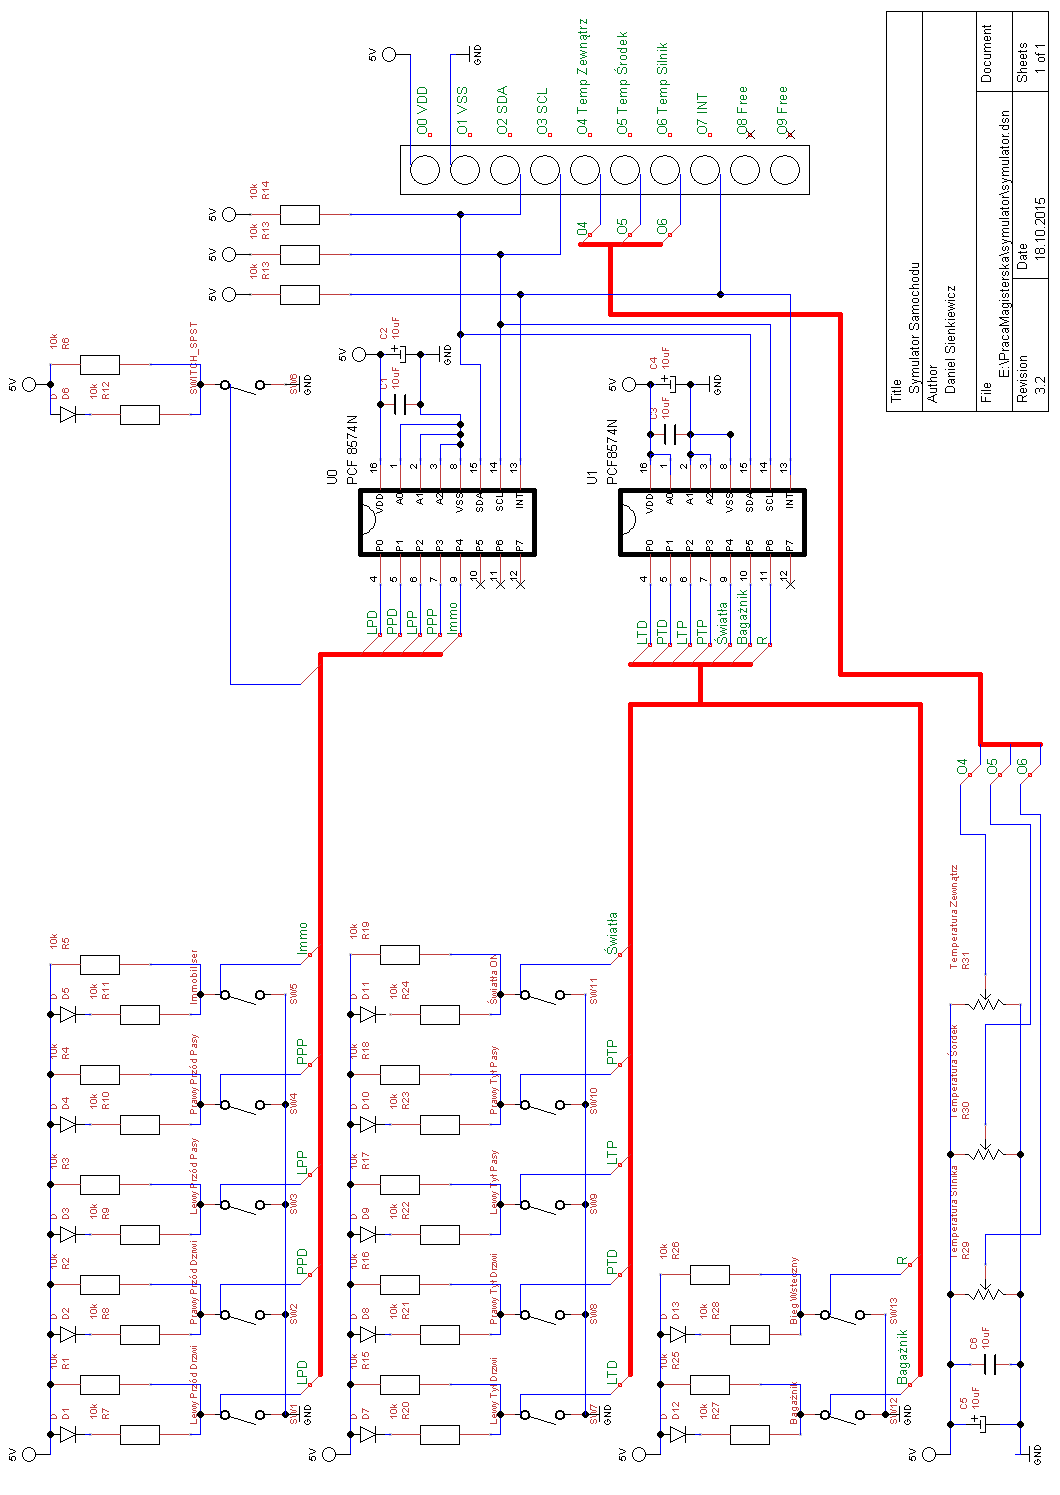
\includegraphics[height=0.6\textheight]{images/symulator.png}
    \caption{Schemat elektryczny symulatora samochodu}
    \source{Opracowanie własne}
\end{figure}

\section{Dalsze kroki oraz propozycje}
schemat blokowy z BAJERAMI i wybrane to co zrobię
%================KONIEC IMPLEMENTACJA=====================

\summary
TO DO

\appendix
\chapter{Karty Katalogowe}
Katalog \emph{datasheets} zawiera karty katalogowe użytych podzespołów
\chapter{Porównanie dostępnych na rynku mikro kontrolerów}
\begin{table}[!tbh]
\begin{tabular}{|c|c|c|c|} \hline
 & Intel Galileo & Raspberry Pi (Model B) & Arduino Uno \\ \hline
Wymiary & 10cm x 7cm  & 85.60mm x 56mm x 21mm & 5.59cm x 16.5cm \\ \hline
Procesor & Intel Quark X1000 & Broadcom BCM2835 & ATmega328 \\ \hline
Taktowanie &	400MHz	& 700MHziv & 16 MHz\\ \hline
Cache &	16 KB & 32KB L1 cache, 128KB L2 cache & - \\ \hline
RAM &	512 SRAm & 512 SRAM & 2 kB \\ \hline
Analog I/O	& 6 & 17 & 6 \\ \hline
Digital I/O	& 14 & 8 & 14 \\ \hline
PWM	& 6 & 1 & 6 \\ \hline
\end{tabular}
\caption{Specyfikacja dostępnych na rynku mikro kontrolerów}
\source{\url{http://eu.mouser.com/applications/open-source-hardware-galileo-pi/}}
\source{\url{http://botland.com.pl/arduino-moduly-glowne/1060-arduino-uno-r3.html}}
\end{table}
\chapter{Programy}
Katalogi \emph{Galileo, PCF8574N} zawierają kod źródłowy oprogramowania stworzonego na potrzeby pracy. 

\noindent Katalog \emph{Galileo} zawiera oprogramowanie mikrokomputera Intel\cite{einstein} Galileo.

\noindent Katalog \emph{PCF8574N} zawiera oprogramowanie I/O Expander PCF8574N.

\bibliographystyle{unsrt}
\bibliography{sample}

\listoftables

\listoffigures

\oswiadczenie

\end{document}
